%\documentclass[a4paper]{fhnwreport} %Legt grundlegende Formatierungen wie Schriftarten, Ort Seitenzahlen etc. fest.
%
%\graphicspath{{./graphics/}}%Change according to graphics folder!
%
%\begin{document}

\section{Software}
Die Anforderung des Auftraggebers beinhaltet, dass die Kommunikation zwischen Sensorplatine und Meldezentrale über die Powerline erfolgt und keine zusätzliche Leitung beanspruchen darf. Für die drahtlose Übertragung war die Idee die Kommunikation über ein kabelloses System, wie Bluetooth oder Wireless zu verwenden. Diese Idee wurde aufgrund der unbekannten Distanzen zwischen der Sensor- und Meldeplatine verworfen. Für diese Einkopplung wird ein fertiger Transceiver und ein Kommunikationsprotokoll verwendet. Die Kommunikation zwischen Mikrocontroller und Transceiver wird mit UART realisiert. Es wird auf der Sensorplatine ein Mikrocontroller ATMega328P verwendet.


\subsection{Sensorplatine}
Die Aufgabe der Sensorplatine besteht aus der Verarbeitung der gemessenen Daten und der Übermittlung der Daten. In der Abbildung \ref{fig:Software_Flussdiagramm_Sensorplatine} ist der Verlauf dieser Verarbeitung ersichtlich.

\begin{figure}[htbp] 
  \centering
     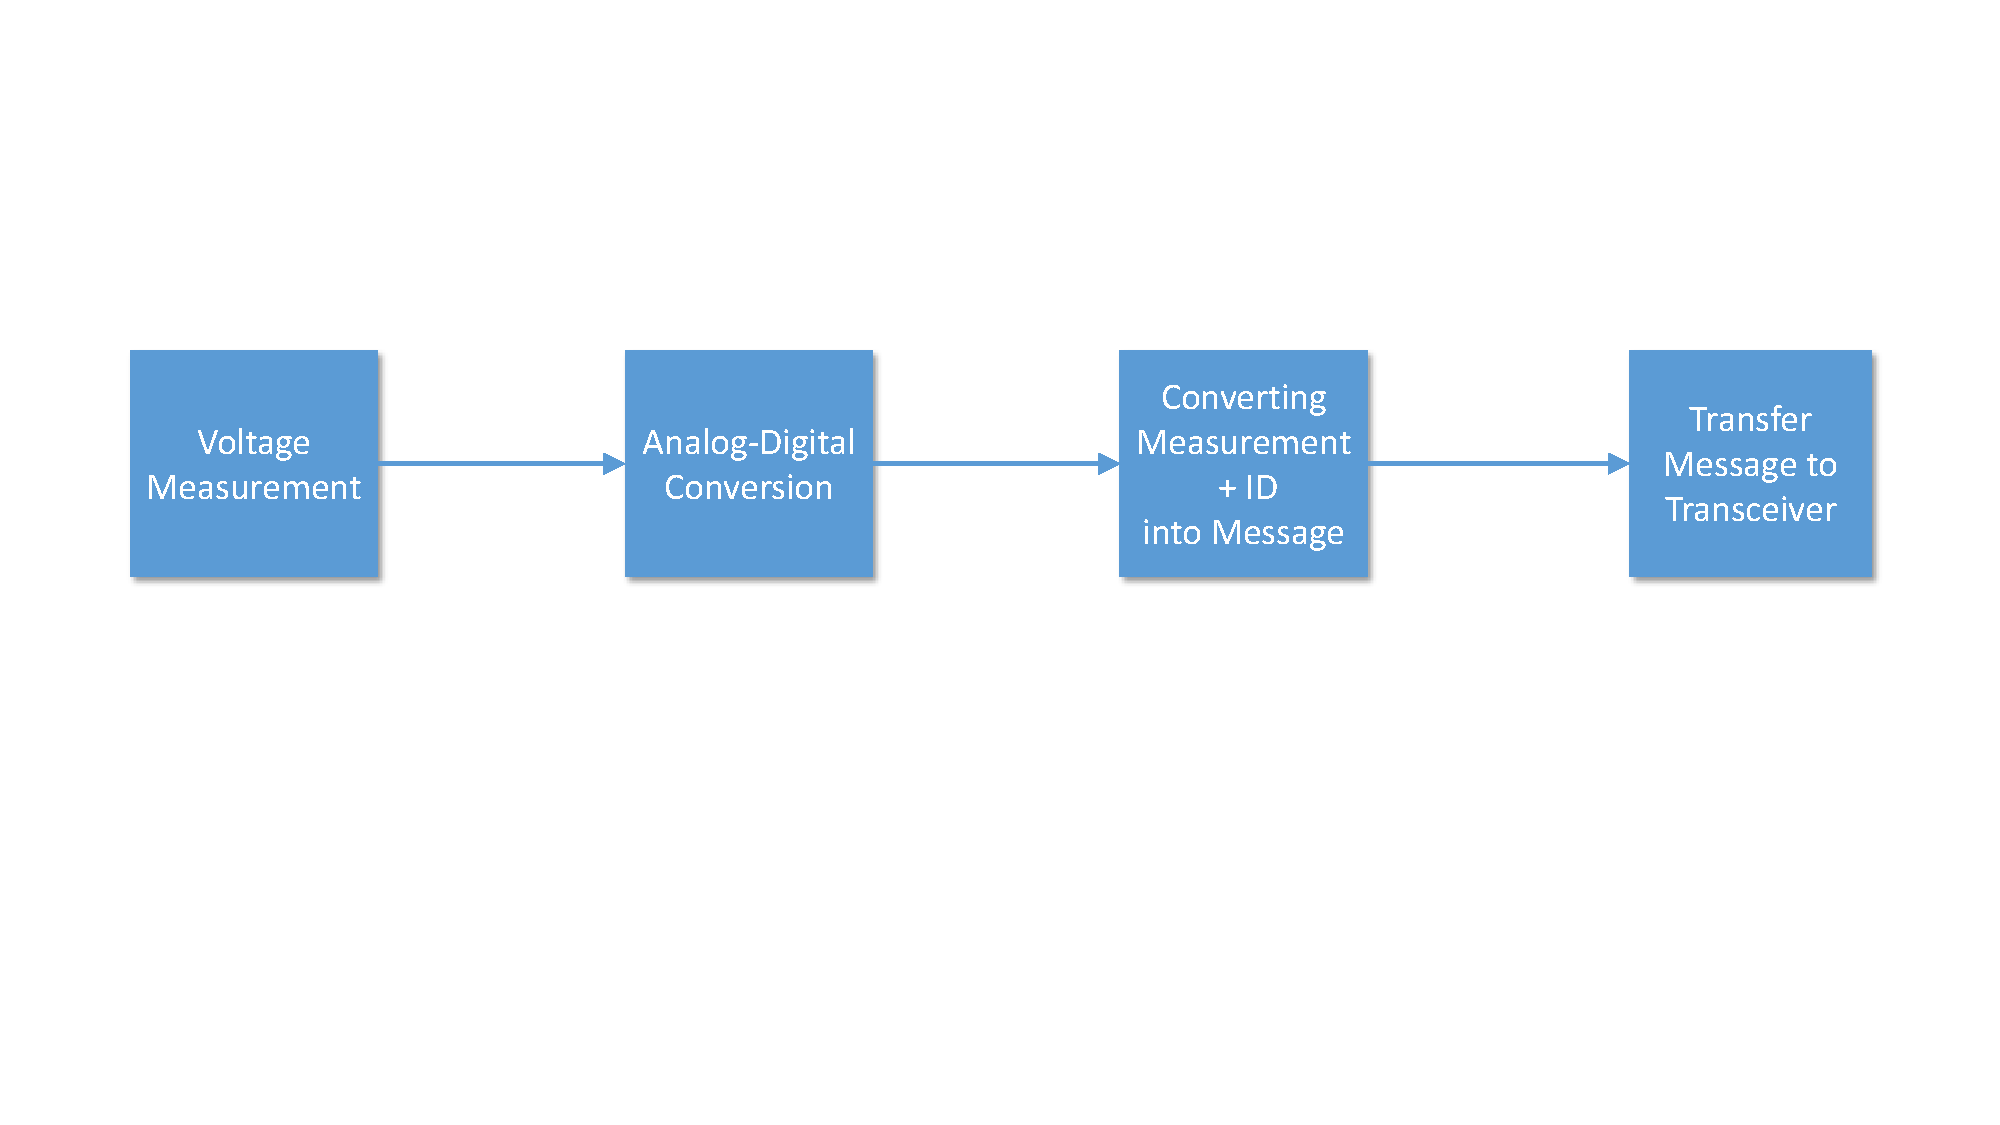
\includegraphics[width=1\textwidth]{graphics/Sensorplatine_Flussdiagramm}
  \caption{Flussdiagramm Verlauf Programm Sensorplatine}
  \label{fig:Software_Flussdiagramm_Sensorplatine}
\end{figure}

Im ersten Schritt in der Abbildung \ref{fig:Software_Flussdiagramm_Sensorplatine} werden von der Messung die Daten eingelesen und in verwendbare Datentypen gespeichert. Die Kommunikation zum Transceiver wird über eine serielle asynchrone Schnittstelle stattfinden. Der Modulator wird die Messdaten auf die Leitung, Powerline Communication, induktiv einkoppeln. \\ Die Kommunikation soll unidirektional sein. Das Problem der Kollisionen soll wie folgt vermieden bzw. verringert werden: Innerhalb einer Stunde werden die Daten von allen Modulen mehrere Male gesendet, wobei die Verzögerung zwischen zwei Sendeversuchen einen statischen und einen zufälligen Teil enthält. Dies verringert die Wahrscheinlichkeit, dass zwei Kollisionen hintereinander auftreten.
Der Empfänger prüft die Vollständigkeit der Daten anhand einer Checksumme (CRC).

\subsection{Kontrollplatine}
Die Meldeplatine wird die Zentrale aller Sensorplatinen sein. Sie hat die Aufgabe den Betrieb der Anlage zu überwachen sowie die gesammelten und übermittelten Daten der Sensorplatinen auszuwerten. Für einen detektierten Fehler wird ein Relaiskontakt geschaltet und die fehlerhafte Stelle auf dem Display eingeblendet. Der gesamte Verlauf ist in Abbildung \ref{fig:Scheme_report_board} dargestellt.

\begin{figure}[h!] 
  \centering
     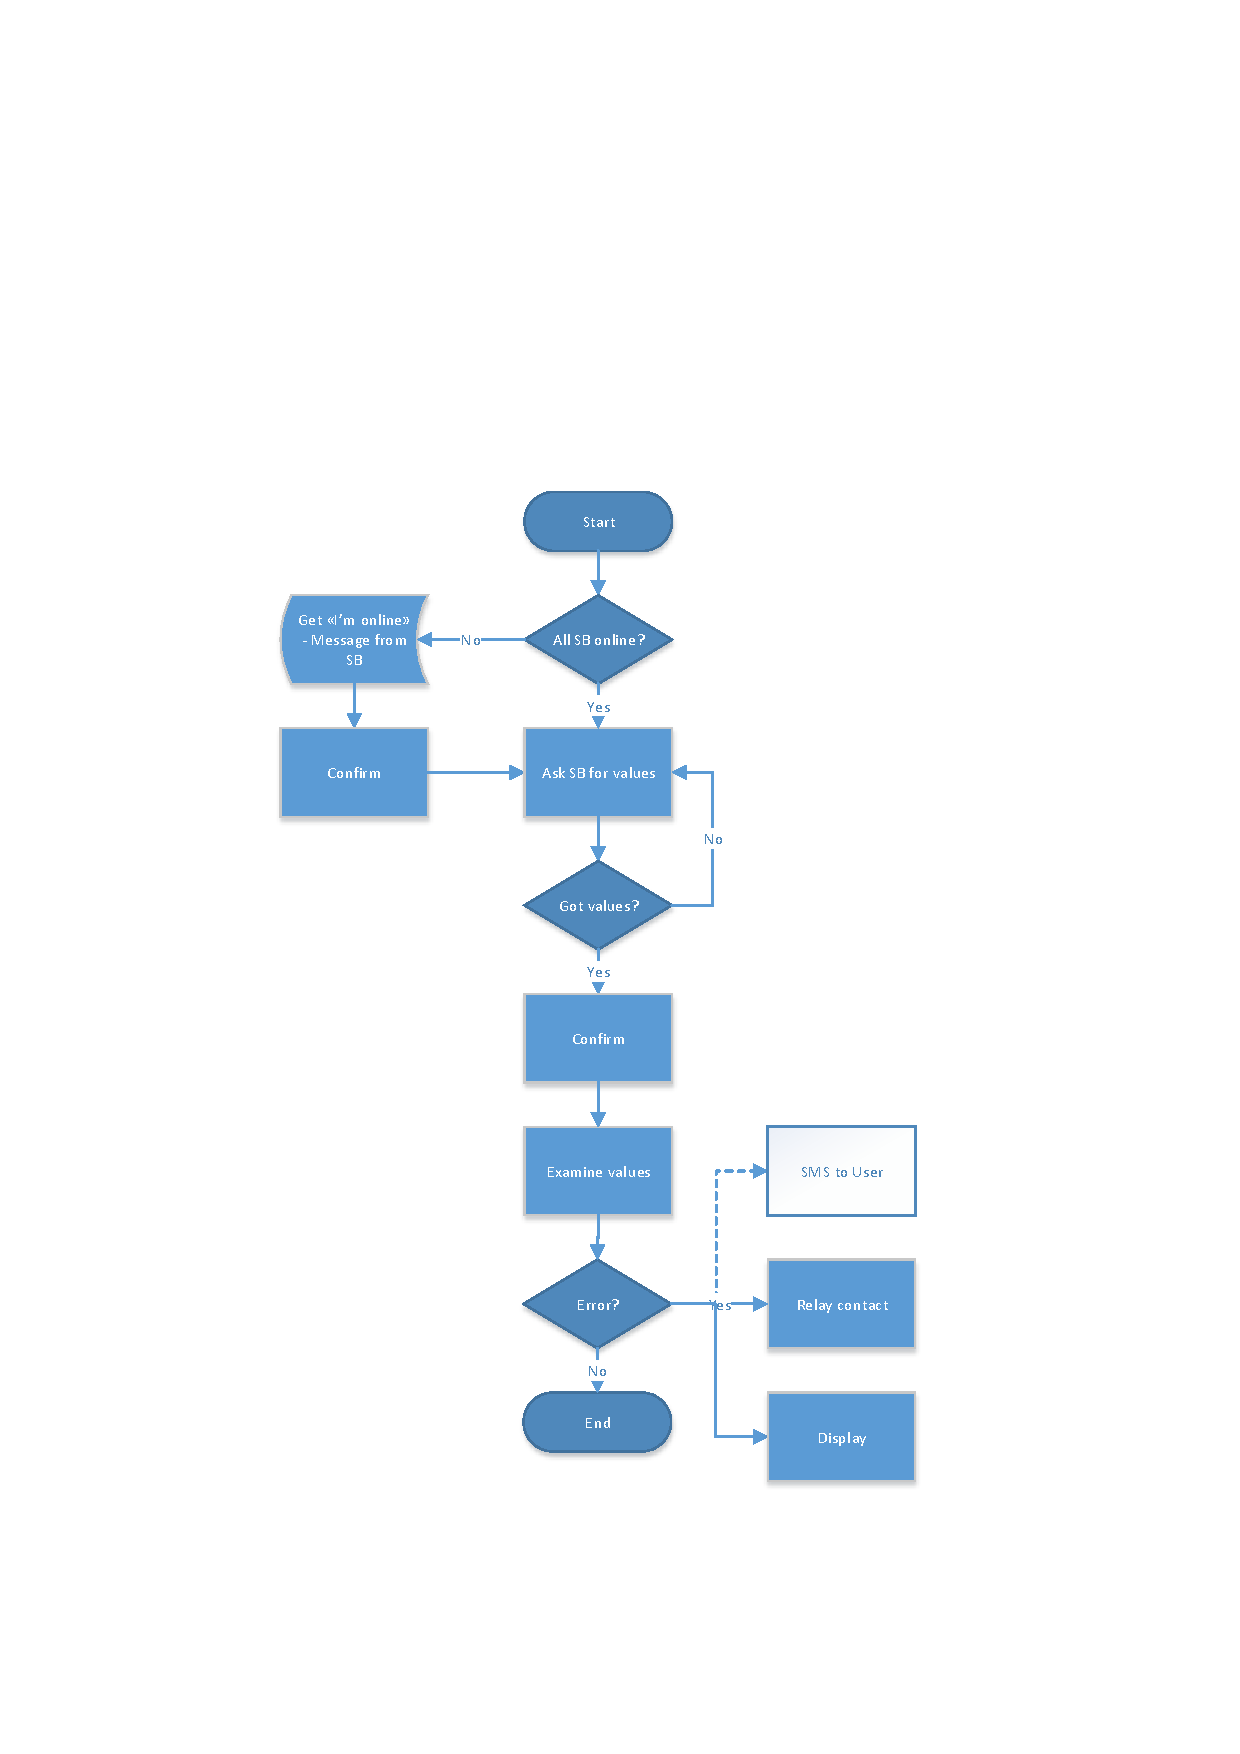
\includegraphics[width=0.5\textwidth]{graphics/Scheme_report_board}
  \caption{Flussdiagramm Verlauf Programm Meldeplatine}
  \label{fig:Scheme_report_board}
\end{figure}

\newpage

Damit die Meldeplatine die Anlage überwachen kann muss sichergestellt werden, dass alle Messwerte empfangen werden. Zu diesem Zweck erstellt die Meldeplatine bei der ersten Inbetriebnahme ein Register der Sensorplatinen (``Build register''). Danach beginnt sie die Messungen der Sensorplatinen zu empfangen (``Receive values'') und anschliessend auszuwerten (``Examine values''). Es besteht die Möglichkeit, dass eine Sensorplatine zur Zeit offline ist, fehlerhaft oder gleichzeitig mit einer anderen Sensorplatine Informationen sendet. Falls dies der Fall sein sollte, kommt es zu einer Warnung. Kommunizieren nach einer Wartezeit immernoch nicht alle Sensorplatinen richtig, kommt es zu einem Fehler, welcher einen Relaiskontakt betätigt und eine Meldung auf dem Display ausgibt.\\
Der Algorithmus für die Datenauswertung funktioniert nach dem arithemtischen Mittel. Es sagt aus, dass alle Datenpunkte addiert geteilt durch die Anzahl Datenpunkte einen Mittelwert ergibt. Weicht ein einzelner Datenpunkt stark vom Mittelwert ab, entspricht dieser einer Warnung. Um anschliessend das fehlerhafte Modul zu lokalisieren bekommt jede Sensorplatine eine Identifikationsnummer, die alle in einem Anlagenschema abgelegt sind.\\

Die Situation ``Nacht'' wird anhand des Vergleichs von Mittelwert und dem minimalen Spannungslevel (12V) ermittelt, sodass in dieser Zeit keine Fehler ausgegeben werden.


\subsection{Mittelwertbildung}
Die Mittelwertbildung beginnt bereits bei der Sensorplatine. Sie misst mehrmals in der Minute die Spannung, bildet einen gleitenden Mittelwert und speichert diesen. Die Sensorplatinen senden dann mehrmals stündlich ihren Spannungs-Mittelwert an die Meldeplatine. Die Meldeplatine kontrolliert in einem Register, ob auch alle Sensorplatinen einen Spannungs-Mittelwert gesendet haben. Ist das Register nach einer Stunde komplett, rechnet die Meldeplatine über alle Messwerte den gesamten Mittelwert.\\
Falls das Register nicht komplett ist, ist das ein möglicher Fehler, der aber verzögert ausgegeben wird, damit die Sensorplatine Zeit hat ihren Messwert nochmals zu senden.
%\end{document}